% ==============================================
\section{Motivating Examples and Tool Features}
\label{sec:motivation}
% ==============================================
%\begin{figure*}
%\centering
%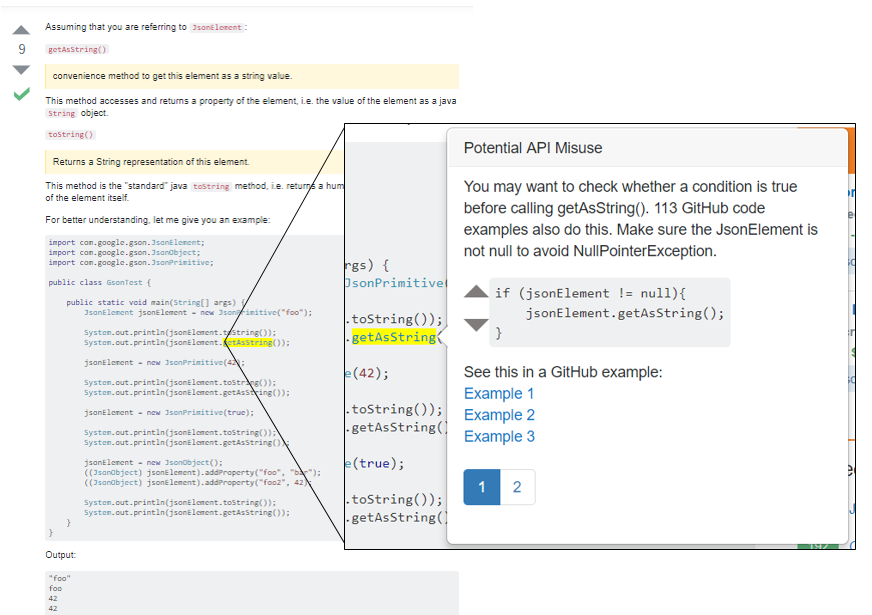
\includegraphics[width=0.6\textwidth]{json_ex1_context.PNG}
%  \vspace{.1in}
%  \caption{A code snippet that does not properly check {\tt JsonElement.getAsString}.\protect\footnotemark}
%  \label{fig:so_example}
%\end{figure*}
%
%\begin{figure*}[t!]
%\centering
%  \begin{subfigure}[t]{0.48\textwidth}
%  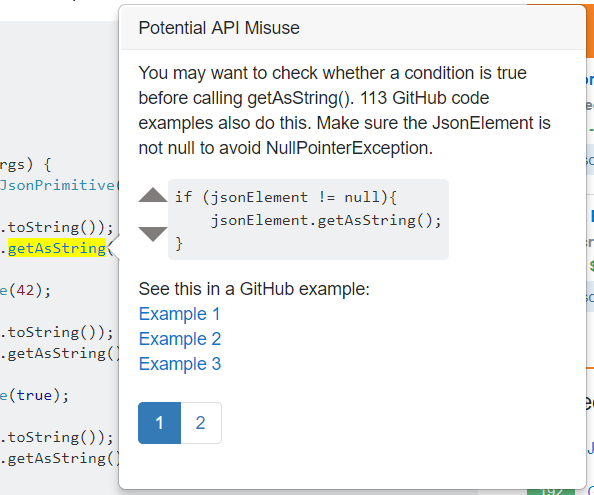
\includegraphics[width=\textwidth, height=6cm]{json_ex2.PNG}
%  \caption{A page describing a way to avoid a {\tt NullPointerException} by checking whether the {\tt JsonElement} object is null. \todo{should I still include this figure when it's sort of subsumed by Figure~\ref{fig:so_example}?}} 
%  \label{fig:page1}
%  \end{subfigure}
%  \hspace{0.02\textwidth}
%  \begin{subfigure}[t]{0.48\textwidth}
%  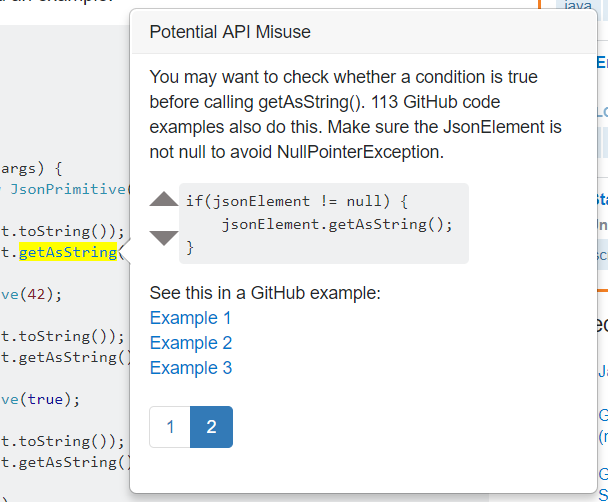
\includegraphics[width=\textwidth, height=6cm]{json_ex3.PNG}
%  \caption{A page describing a way to avoid a {\tt ClassCastException} by checking whether the {\tt JsonElement} object is a primitive.}
%  \label{fig:page2}
%  \end{subfigure}
%  \hfill
%  \vspace{0.02\textwidth}
%\caption{The two pages of a popup generated on {\tt JsonElement.getAsString}.\todo{Can we also show how many users like or dislike the violations in the popup window? Since we don't have any real users, maybe we need to create some artificial numbers for the demonstration purpose.}}
%\label{fig:features}
%\end{figure*}

\begin{figure}
\centering
\includegraphics[width=0.49\textwidth]{github-example-v2.pdf}
  \vspace{.1in}
  \caption{{\tool} will redirect the programmer to a highlighted concrete code example in GitHub that follows the correct API usage pattern, when she clicks on one of the three GitHub example links in the pop-up window.\protect\footnotemark}
  \label{fig:github}
\end{figure}

\footnotetext{\url{https://goo.gl/YHo1UM}}

Suppose Alice needs to read attribute values from a {\ttt JSON} message using Google's Gson library, which she is not familiar with. Alice finds a Stack Overflow answer post that reads a specific {\ttt JSON} message posted in the corresponding question post.\footnote{\url{https://stackoverflow.com/questions/29859683/assistance-with-json-from-url}} Though the answer post is accepted as the correct answer, this post does not properly use {\ttt JsonElement.getAsString} (line 7 in the snippet in Figure~\ref{fig:screenshot}), which gets the {\ttt string} value of a {\ttt JSON} element. For example, if the requested attribute does not exist in the {\ttt JSON} message, the preceding API call, {\ttt JsonObject.get} (line 2) may return {\ttt null}, which consequently leads to {\ttt NullPointException} when calling {\ttt getAsString} on the returned object. If Alice puts too much trust on this example, she may inadvertently follow a suboptimal solution, which may crash her program in some corner cases. 

Alice cannot easily recognize this potential limitation in the given Stack Overflow post. She may have to manually investigate many other posts till finding a code example with ideal API usage. In practice, however, programmers often examine a handful of search results due to the limited time and attention~\cite{brandt2009two, starke2009working, duala2012asking}. {\tool} frees Alice from this manual investigation labor by constrasting a Stack Overflow post with common API usage patterns learned from over 380K GitHub repositories. {\tool} then highlights the API calls that have potential API usage violations in the Stack Overflow post. When Alice clicks on the highlighted API call, {\tool} generates a pop-up window with detailed descriptions about the API usage violation, as shown in Figure~\ref{fig:screenshot}.

{\bf API misuse description.} To help Alice understand a detected API usage violation, {\tool} translates the violation to a short natural language description (see \ding{172} in Figure~\ref{fig:screenshot}). From  the short warning message, Alice learns that she should check whether the {\ttt JsonElement} object is {\ttt null} before calling {\ttt getAsString}. Furthermore, {\tool} shows how many GitHub examples also follow the API usage pattern that the Stack Overflow post violates. This quantification of how many GitHub code examples are consistent with the shown snippet can provide an additional argument about the prevalence of API usage patterns in real-world projects and help Alice build confidence on the detected violations.

\begin{figure}
\centering
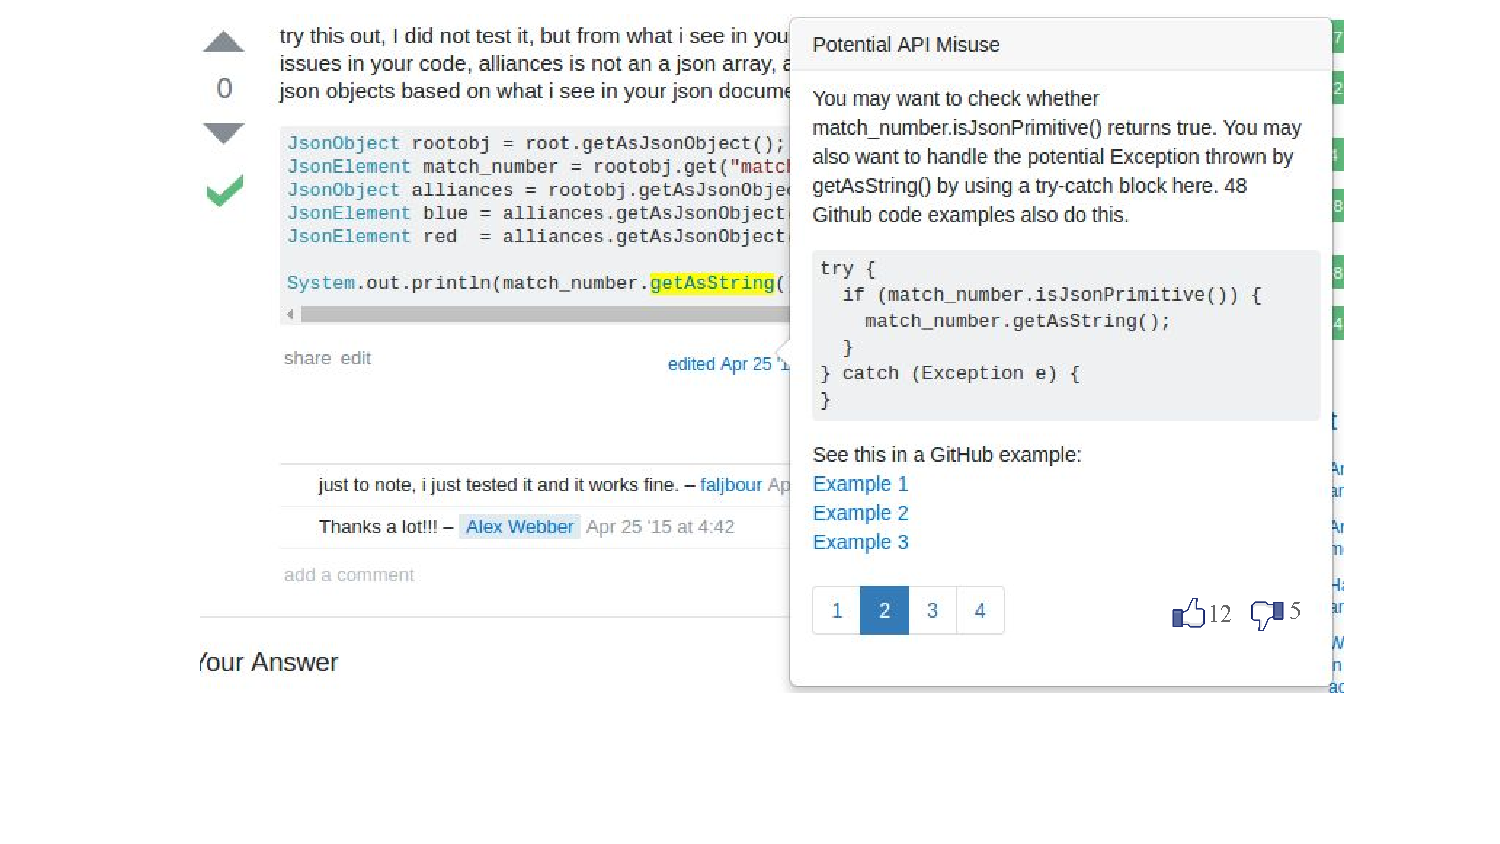
\includegraphics[width=0.5\textwidth]{soap-v3-2.pdf}
  \vspace{.1in}
  \caption{Another API usage warning that reminds programmers to check whether the {\ttt JsonElement} object represents a {\ttt JSON} primitive value by calling the {\ttt isJsonPrimitive} method. It also suggests to catch potential exceptions thrown by {\ttt getAsString}.}
  \label{fig:screenshot2}
\end{figure}

{\bf Fix suggestion.} To demonstrate how to fix the violation, {\tool} suggests a fix that follows the correct API usage pattern and corrects the violation in the original Stack Overflow post. The fix is generated based on the context of the Stack Overflow post to mitigate the mind gap between the original post and the fix. For example, the {\ttt JsonElement} variable in the fix is named as the corresponding variable, {\ttt match\_number} in the original post (see \ding{174} in Figure~\ref{fig:screenshot}). 

\begin{figure*}[!th]
\centering
\includegraphics[width=0.8\textwidth]{maple-extension-v3.pdf}
\vspace{.1in}
\caption{An overview of {\tool}'s architecture}
\label{fig:arch}
\end{figure*}

{\bf Demonstrative GitHub examples.} {\tool} provides three demonstrative GitHub examples that follow the same API usage pattern (see \ding{175} in Figure~\ref{fig:screenshot}). Alice is curious about how other programmers use {\ttt JsonElement.getAsString} in real-world projects so she clicks on the link of the first GitHub example. {\tool} redirects Alice to a GitHub page and automatically scrolls down to the Java method where {\ttt JsonElement.getAsString} is called. {\tool} also highlights the example so Alice can easily find it, as shown in Figure~\ref{fig:github}. The addition of concrete GitHub examples can aid Alice in understanding how the API of interest is used in real-world projects. 


{\bf Multiple API usage violations.} If a method call in a Stack Overflow post violates multiple API usage patterns, {\tool} describes these violations in separate pages in the pop-up window. For example, the method call, {\ttt getAsString} in Figure~\ref{fig:screenshot} violates four API usage patterns (see \ding{176} in Figure~\ref{fig:screenshot}). Figure~\ref{fig:screenshot2} shows the second violated pattern and suggests Alice to check whether the {\ttt JsonElement} object is primitive before calling {\ttt getAsString}. Otherwise, {\ttt getAsString} will throw {\ttt ClassCastException}. {\tool} also suggests Alice to wrap {\ttt getAsString} with a try-catch block to handle other potential exceptions such as {\ttt IllegalStateException}. Alice notices that this pattern is supported by 48 GitHub examples, while the pattern in Figure~\ref{fig:screenshot} is supported by 119 GitHub examples.

{\bf User feedback.} After seeing concrete GitHub examples as well as the number of GitHub supports for each pattern, Alice can infer that the {\ttt null} check in Figure~\ref{fig:screenshot} is necessary and is more common than the primitive check in Figure~\ref{fig:screenshot2}. She upvotes the pattern by clicking on the ``thumbs-up'' button to notify other users that this detected violation is helpful to her (see \ding{177} in Figure~\ref{fig:screenshot}). %The server also updates the vote of this pattern based on Alice's feedback at the back end.

%\begin{figure*}[t!]
%\centering
%  \begin{subfigure}[t]{0.48\textwidth}
%  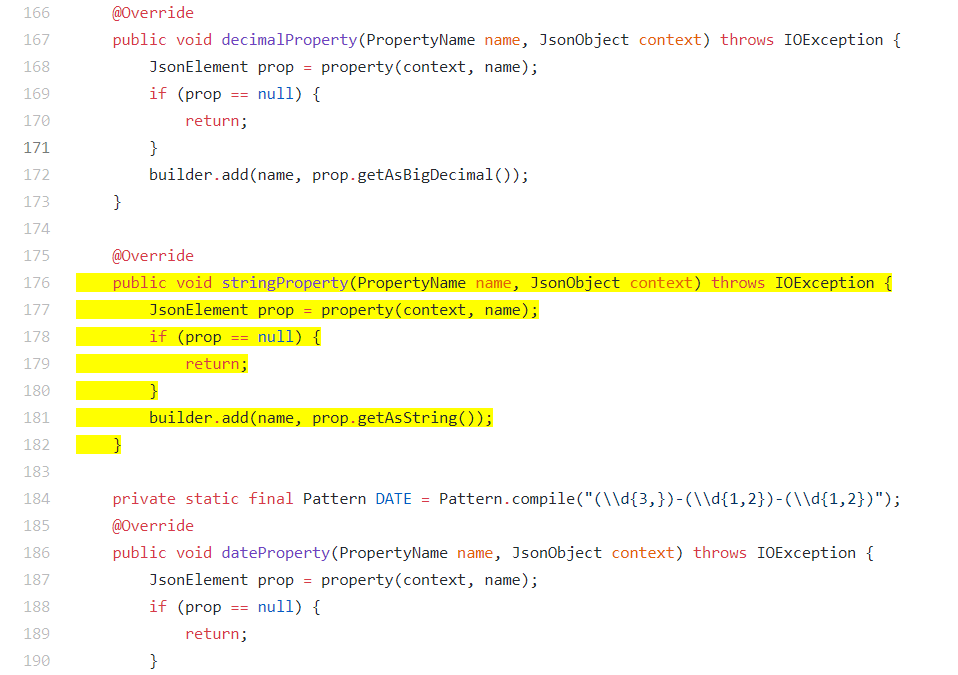
\includegraphics[width=\textwidth]{json_null_gh2_context.PNG}
%  \caption{The second GitHub example for Figure~\ref{fig:page1} in the context of its GitHub file.\protect\footnotemark} 
%  \vspace{.1in}
%  \label{fig:github1}
%  \end{subfigure}
%  \hfill
%  \begin{subfigure}[t]{0.48\textwidth}
%  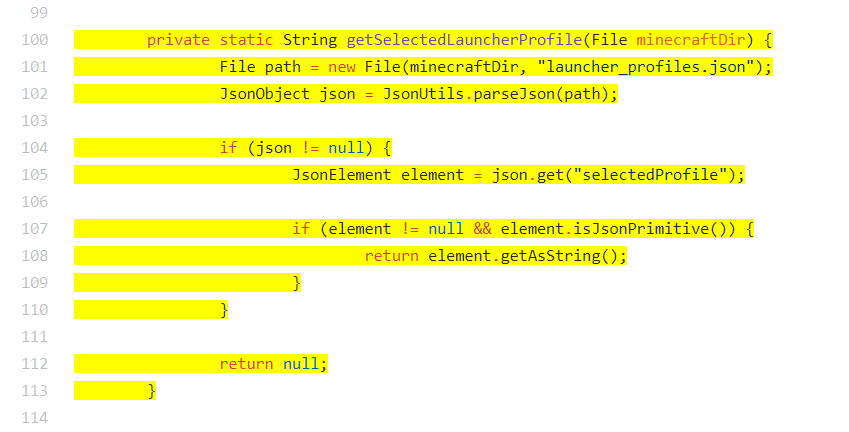
\includegraphics[width=\textwidth]{json_primitive_gh1.PNG}
%  \caption{The first GitHub example for Figure~\ref{fig:page2}.\protect\footnotemark}
%  \vspace{.1in}
%  \label{fig:github2}
%  \end{subfigure}
%  \hfill
%\caption{The GitHub examples redirected to from the links provided in the popup, highlighted by the Chrome extension.\todo{The snapshot only shows the highlighted code. Is there a better way to give paper reviewers some context that the highlighted code is from GitHub and that the code is selectively highlighted by our tool instead of by GitHub?}}
%\label{fig:github_examples}
%\end{figure*}

%\begin{figure}
%\centering
%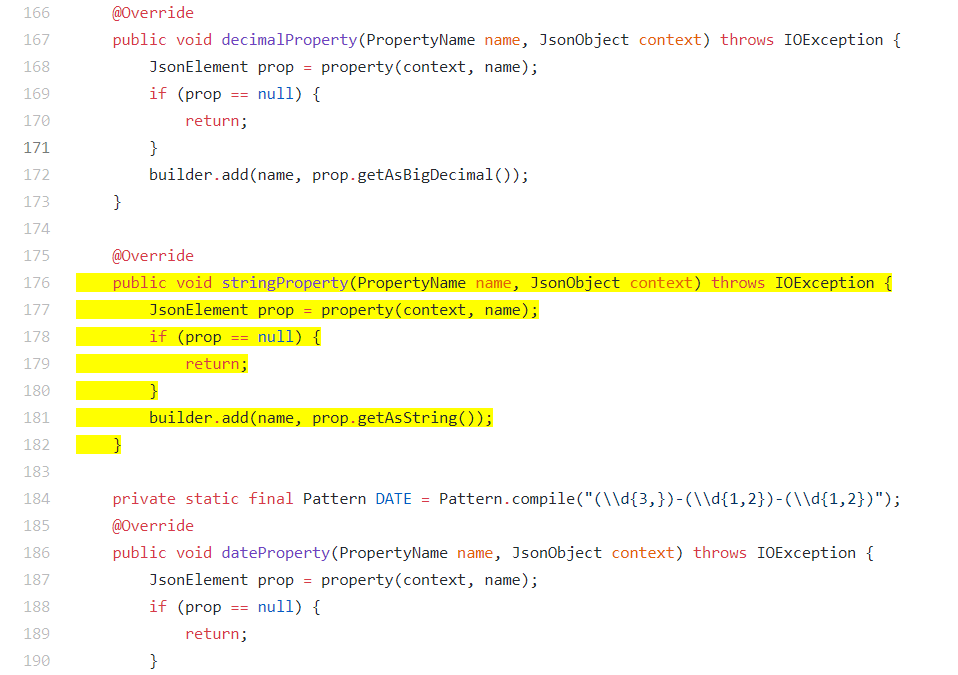
\includegraphics[width=0.48\textwidth]{json_null_gh2_context.PNG}
  %\caption{The GitHub example that a link from Figure~\ref{fig:page1} redirects to, highlighted by the Chrome extension.\protect\footnotemark} 
  %\label{fig:github_examples}
%\end{figure}

%https://github.com/asakusafw/asakusafw/blob/cad94753128bd3168e23c0539cc55c7e5a653dbd/asakusa-test-data-provider/src/main/java/com/asakusafw/testdriver/json/JsonObjectDriver.java
%\footnotetext{http://tinyurl.com/JsonObjectDriver}

%https://github.com/Spoutcraft/Spoutcraft/blob/5cbbc2b07edaf4194a36130a7e74321e5b30ace0/src/main/java/com/prupe/mcpatcher/Config.java
%\footnotetext{http://tinyurl.com/SpoutcraftConfig}